\section{Propuesta}
\subsection{Salas de reunión}
En las salas de reunión se pudo analizar que el tiempo de reverberación no es el mejor para su 
utilización según la norma DIN$18041$, por lo que con esta solución se buscará disminuirlo, 
mejorando la inteligibilidad y la claridad del habla.\\
Para esto se sugiere la aplicación de un panel de volcanita ranurado con lana de vidrio, con un 
plenum de $20$ cm y lana de vidrio de $6$ cm, esto en un área del cielo donde la superficie en la sala 1 sería de  $12.5$ $m^2$ 
y de $9$ $m^2$ en la sala $2$, como se puede observar en la figura \ref{fig:propuesta_reunion1} y \ref{fig:propuesta_reunion2}.

\begin{figure}[H]
    \centering
    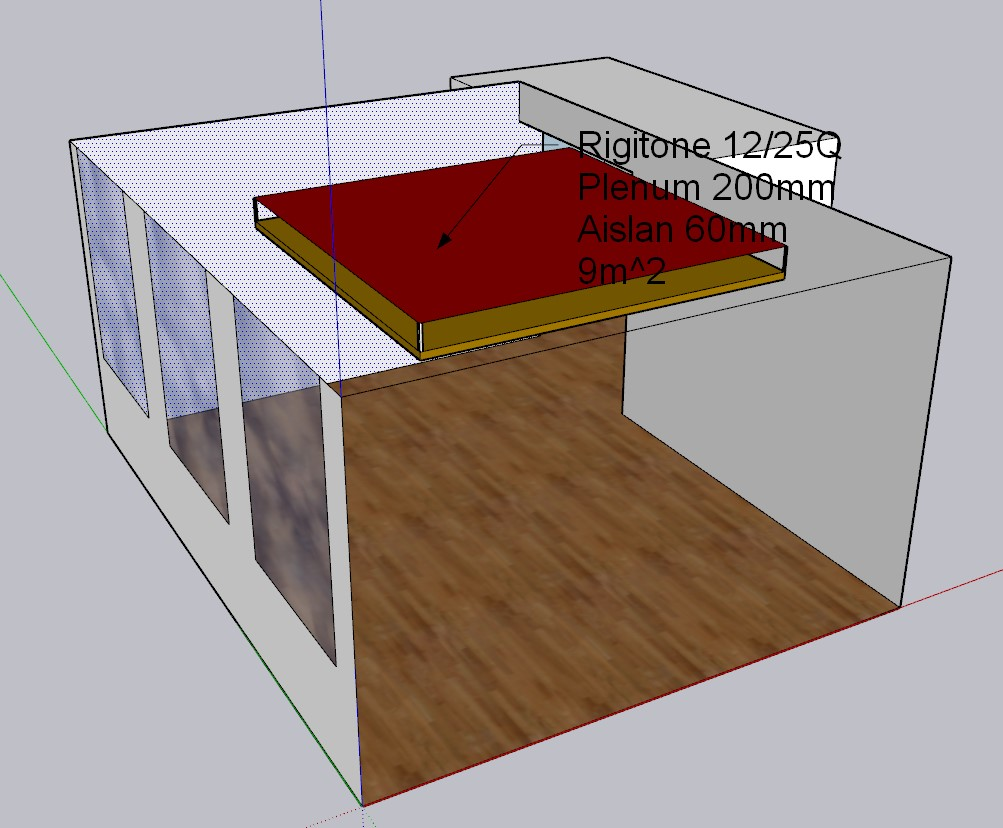
\includegraphics[width=10cm]{Imagenes/Propuesta/propuesta_reunion1.jpg}
    \caption{Propuesta de acondicionamiento en sala de reunión 1}
    \label{fig:propuesta_reunion1}
\end{figure}

\begin{figure}[H]
    \centering
    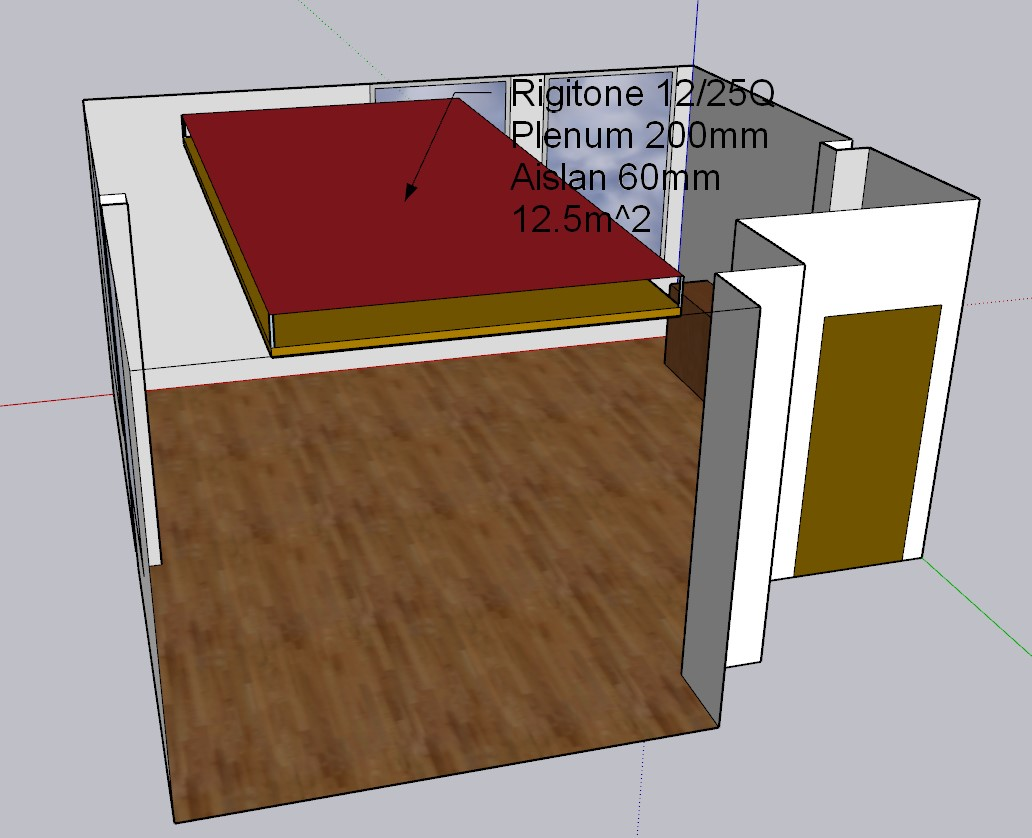
\includegraphics[width=10cm]{Imagenes/Propuesta/propuesta_reunion2.jpg}
    \caption{Propuesta de acondicionamiento en sala de reunión 2}
    \label{fig:propuesta_reunion2}
\end{figure}

El coeficiente de absorción acústica del conjunto de materiales indicados se indican en la tabla \ref{tab: coef abs volcanita Rigitone}
\begin{table}[H]
    \centering
    \begin{tabular}{|lllllll|}
    \hline
    \multicolumn{7}{|c|}{\textbf{12/25 Q}} \\ \hline
    \multicolumn{1}{|l|}{Plenum} & \multicolumn{6}{c|}{200 mm} \\ \hline
    \multicolumn{1}{|l|}{Aislan} & \multicolumn{6}{c|}{60  mm} \\ \hline
    \multicolumn{1}{|l|}{Frecuencia Hz} & \multicolumn{1}{l|}{125 Hz} & \multicolumn{1}{l|}{250Hz} & \multicolumn{1}{l|}{500 Hz} & \multicolumn{1}{l|}{1 KHz} & \multicolumn{1}{l|}{2KHz} & 4KHz \\ \hline
    \multicolumn{1}{|l|}{$\alpha$} & \multicolumn{1}{l|}{0.60} & \multicolumn{1}{l|}{0.90} & \multicolumn{1}{l|}{0.95} & \multicolumn{1}{l|}{0.90} & \multicolumn{1}{l|}{0.80} & 0.75 \\ \hline
    \end{tabular}
    \caption{Coeficiente de absorción de Volcanita acústica Rigitone}
    \label{tab: coef abs volcanita Rigitone}
\end{table}  

\subsection{Sala de ensayo}
Para la sala de ensayo se recomienda extraer el material absorbente que se instaló, cambiando así el tiempo de reverberación favorablemente para el uso que le da al recinto.
%agregar imagen de sala sin paneles.